\section{Analyse af problemområde}

Ud fra systemdefinitionen i \myref{Sysdef} ved vi, at systemet skal holde styr på følgende:

\begin{itemize}[noitemsep,nolistsep]
	\item Tilbud
	\item Varer
	\item Indkøbslister
	\item Opskrifter
\end{itemize}

Med disse informationer kan systemet hjælpe brugeren til at finde billige varer i bestemte butikker og eventuelt anbefale opskrifter, der bruger disse tilbudsvarer.
I de følgende afsnit vil disse emner blive beskrevet vha. klassebeskrivelser, en hændelsestabel, og et klassediagram.

\subsection{Klasser}
I dette afsnit vil vi analysere klassernes sammenhæng, derudover vil yderligere klasser blive tilføjet, hvis det findes nødvendigt.

\begin{description}
\item[Vare]\hfill\\
En vare indgår i opskrifter, og indkøbslister.
Når man laver sin indkøbsliste, kan man vælge varer man vil købe, og tilføje dem til indkøbslisten.
Desuden kan en vare have et antal tilbud, hvilket betyder, at der også skal laves en relation til tilbudsklassen.

\item[Tilbud]\hfill\\
Når der kommer nye varer på tilbud, modelleres disse og kobles, vha. en association, til varer.

\item[Opskrift]\hfill\\
En opskrift har en liste over ingredienser, hvilket altså er varer samt mængden af varen.
I interviewene i \myref{section:interview2}, blev det nævnt, at brugerne gerne ville kunne vurdere en opskrift og dermed få anbefalet yderligere opskrifter, som minder om denne.
For at kunne lave vurderinger, skal der laves en vurderingsklasse.

\item[Vurdering]\hfill\\
En vurdering med tal gives for at rangere opskrifter. 
Vurderingen danner også grundlag for, at systemet kan anbefale opskrifter.

\item[Anbefaling]\hfill\\
En anbefaling, af en opskrift, kan gives til personer, når de har givet positive vurderinger af andre opskrifter, som minder om den vurderede opskrift.

\item[Person]\hfill\\
Personklassen gør det muligt at holde styr på forskellige personer, da disse tilsluttes opskrifter, vurderinger, og indkøbsliter.
Derudover vil en person også have præferencer, for butikker de handler i, samt madvarer.

\item[Indkøbsliste]\hfill\\
Indkøbslister laves af en person, og fyldes op med objekter fra vareklassen.
Indkøbslisterne kan deles imellem flere brugere.
\end{description}


\subsection{Hændelser}\label{handelser}
På baggrund af de nævnte funktionaliteter i prototype interviewene, \myref{section:interview2}, er der fundet forskellige hændelser, relevante for funktionaliteterne.
Ud fra disse laves en hændelsestabel, der beskriver, hvilke klasser forskellige hændelser påvirker.
Formålet med, at identificere hændelserne samt at analysere disse i en hændelsestabel, er at forstå problemområdet bedre.
Derved kan det hjælpe med forståelsen for, hvordan en løsning ville kunne designes, for at afhjælpe de problemer, der findes i problemområdet. 
Desuden kan tabellen hjælpe med strukturen på klasserne.
Hvis to klasser har samme hændelser, kan disse klasser ofte tilpasses under én klasse, og dermed opnås en bedre struktur.

\begin{table}[H]
  \centering
    \colorlet{shadecolor}{gray!40}
    \rowcolors{1}{white}{shadecolor}
      \begin{tabular}{l|lccccccc}
      %\hline
       								& \rot{Tilbud}  & \rot{Indkøbsliste} & \rot{Opskrift} & \rot{Vare} & \rot{Person}& \rot{Vurderinger} \\ \hline
      Vare tilføjet til indkøbsliste&               & +      &          & +     & +     &   \\ 
      Vare fjernet fra indkøbsliste	&              	& +      &          & +     & +     &   \\ 
      Vare aftjekket på indkøbsliste&               & +      &          & +     & +     &   \\ 
      Opskrift valgt ???       		& +             & +      &          & +     & +     &   \\ 
      Tilbud oprettet        		& +            	& +      & +        & +     &       &   \\ 
      Tilbud aktiveret        		& +            	& +      & +        & +     &       &   \\ 
      Tilbud udgået          		& +        		& +      & +     	&       &       &   \\ 
      Vare tilføjet til overvågning & +          	&        &          & +     & +     &   \\ 
      Vare fjernet fra overvågning  & +          	&        &          & +     & +     &   \\ 
      Overvågningsvare på tilbud    & +  			&		 &			& + 	& +		&	\\
      Del indkøbsliste       		&               & +      &          &       & +     &   \\ 
      Indkøbsliste oprettet  		&              	& +      &          &       & +     &   \\ 
      Indkøbsliste slettet  		&             	& +      &          &       & +     &   \\ 
      Vurdering givet				&             	&        & +        &       & +		& + \\
      Anbefaling givet				&				&		 & +		&		& +		& + \\
      
    \end{tabular}
  \caption{Hændelsestabel. Viser hvilket klasser, problemområdets hændelser påvirker.}\label{tabel:haendelsestabel}
\end{table}


Hændelsestabellen, i \myref{tabel:haendelsestabel}, viser både, hvilke hændelser der findes i problemområdet, samt hvilke klasser de påvirker.
Et \textbf{+} beskriver en hændelse, som forekommer højest en gang i et hændelsesforløb.
En \textbf{*} beskriver hændelser, der kan forekomme flere gange i et hændelsesforløb.\citep{OOA&D2001}
På tabellen kan det ses, at klasser der bliver påvirket af mange hændelser, er klasser som \textbf{Indkøbsliste}, \textbf{Vare} og \textbf{Person}.

Ud fra hændelsestabellen kan der dannes et overblik over klassernes interne interaktion, samt hvilke hændelser der involverer hvilke klasser.
Denne information kan vi nu bruge til at lave en struktur over klasserne i problemområdet.

\newpage
\subsection{Struktur}\label{sec:struktur}
\begin{figure}[h]
	\centering
		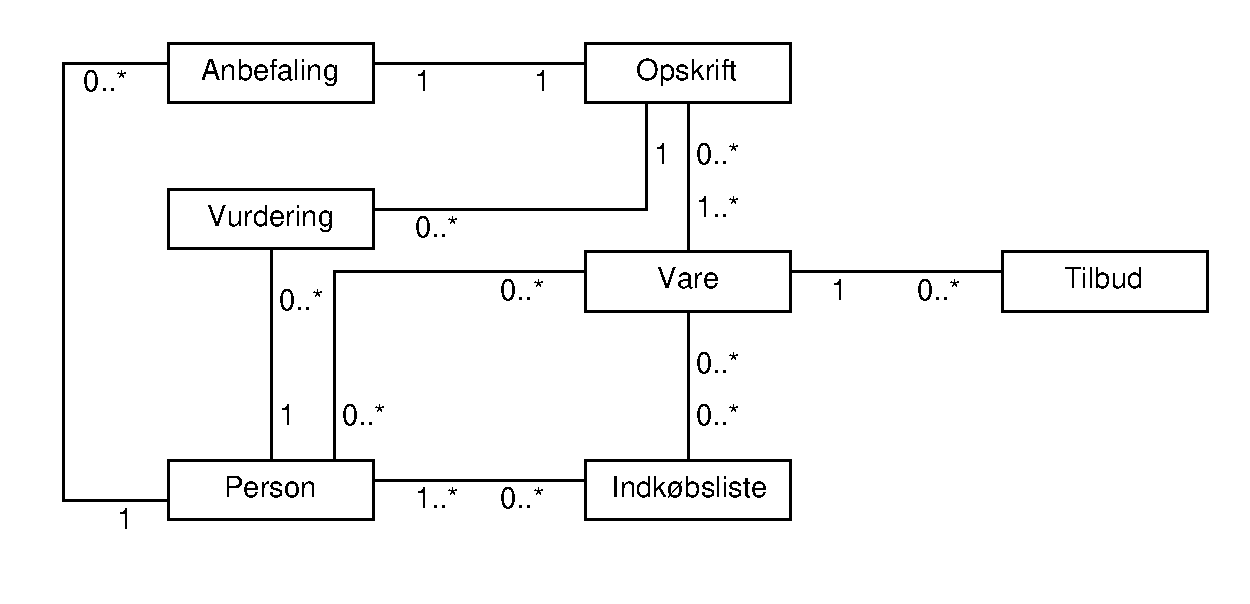
\includegraphics[scale=0.6]{images/Diagrams/klassediagram_model_simple.pdf}
	\caption{Klassediagram over problemområdet.}\label{figur:PDklasse}
\end{figure}

Klassediagrammet, som ses på \myref{figur:PDklasse}, beskriver forholdet mellem de forskellige klasser, som findes i problemområdet.
Diagrammets sammenhænge er dannet ud fra hændelsestabellen, og beskrivelserne af klasserne.

Personer kan lave indkøbslister, og disse indkøbslister kan være ejet og administreret af enten en eller flere personer.
En indkøbsliste kan bestå af nul til mange varer.
En vare kan være på tilbud i mere end en butik og derfor have nul til mange tilbud.
En vare kan desuden indgå i en opskrift og er derfor forbundet med nul til mange.
Desuden har opskrifterne en til mange varer på listen over ingredienser.
Varen kan også være tilføjet til overvågningslisten hos en person, så derfor har personer og varer en nul til mange relation på hinanden.
En person i problemområdet kan give hver opskrift en vurdering, derfor kan personen give nul til mange vurderinger.
En vurdering gives til en opskrift alene, imens en opskrift kan have mange eller ingen vurderinger.
Anbefalinger består af en opskrift, imens personen kan modtage nul til mange anbefalinger.

Ovenstående analyse vil hjælpe til at designe systemets implementering.
Først foretages dog en analyse af anvendelsesområdet, for at undersøge hvad der er muligt at foretage sig i systemet.
